\chapter{Material and Methods}\label{chap:material_and_methods}

\section{Toxicity Data and Processing}\label{sec:invitrodb}
\subsection{ToxCast invitroDB v4.1}
The most recent release of the ToxCast's database, referred to as \emph{invitroDBv4.1}, is an extensive collection of HTS toxicity data ($\sim$\SI{100}{\giga\byte}). This database holds data for 10'196 compounds, each selectively tested across 1'485 assay endpoints. It employs a one-to-many relationship, where a single assay interfaces with numerous endpoints to thoroughly explore a compound's biological effects. An assay constitutes an experimental protocol for high-throughput evaluation of target molecule interactions with compounds, encompassing elements like reagents and response-measuring instruments. Meanwhile, assay endpoints involve specific measurements taken under various conditions and timeframes, delivering a comprehensive understanding of compound-induced biological responses. For an overview of the assay annotation structure, refer to Figure~\ref{fig:assay}.

\begin{figure}  % Placement options: h (here), t (top), b (bottom), p (page)
    \centering
    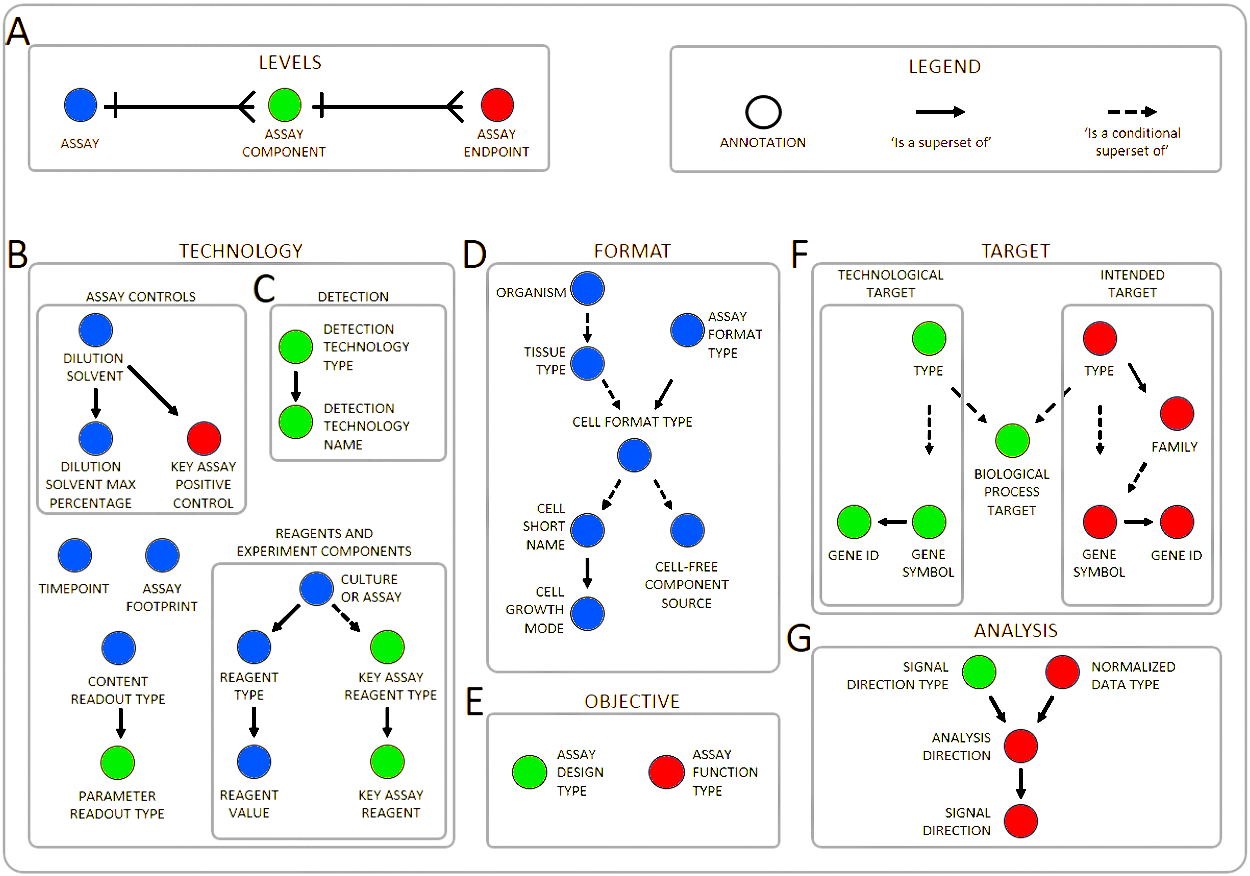
\includegraphics[width=1.0\textwidth]{figures/assay.png}  
    \caption{The annotations for assay endpoints include (A) information for identifying the (color-coded) assay entity, (B) design-related data, (C) details about the target, and (D) information regarding the analysis. These annotations exhibit relationships that can be either one-to-many or conditional, with some dependencies not being applicable in certain cases. This modified figure is sourced from~\cite{userguide}.}
~\label{fig:assay} 
\end{figure}

The assays utilize a range of technologies to assess the impact of chemical compounds on a wide array of biological targets, including individual proteins, nuclear receptor signaling, developmental processes and cellular processes such as mitochondrial health. This resource originates from the collaboration of two prominent institutions: the  U.S. EPA through its ToxCast program and the National Institutes of Health (NIH) via the Tox21 initiative. Using data collected from multiple research labs (refer to Table~\ref{tab:laboratories} in the Appendix), this relational database is accessible to the public and can be downloaded\footnote{\url{https://www.epa.gov/chemical-research/exploring-toxcast-data}, released on Sept 21, 2023} by visiting the official ToxCast website.

\subsection{tcpl v3.0}
The primary ToxCast pipeline is effectively managed through the extensive toolkit offered by the \emph{tcpl}\footnote{\url{https://github.com/USEPA/CompTox-ToxCast-tcpl}} package, which includes a variety of tools for high-throughput screening data management. It enables reproducible concentration-response modeling and populates the \texttt{MYSQL} database, invitroDBv4.1. The multiple concentration screening paradigm intends to pinpoint the bioactivity of compounds, while also estimating their efficacy and potency. In Section~\ref{sec:pytcpl}, we introduce \emph{pytcpl}, a \texttt{Python} reimplementation of the major components that underpin the entire ToxCast pipeline. It should be noted that these components, as presented in the following, are applicable to both tcpl and pytcpl.

\subsection{Efficacy Cutoff}
The evaluation of a compound's bioactivity is significantly influenced by the specific \emph{efficacy cutoff} associated with each assay endpoint, as exemplified for a tested compound in Figure~\ref{fig:concentration_response_series}. It serves as a threshold that differentiates active and inactive compounds, essentially defining the minimum response level of toxicity that is biologically relevant. The process of establishing this threshold involves estimating the noise level in the assay endpoint based on the baseline median absolute deviation (bmad). The bmad is calculated using baseline response values, which are assumed to come from either untreated control wells or test samples from the two lowest concentrations. This calculation is performed just once for the entire assay endpoint.

\subsection{Concentration-Response Series}
Each compound $c_j$ tested within an assay endpoint $a_i$ involves the collection of the respective \emph{concentration-response series (CRS)} denoted as $CRS_{ij}$, showcased in Figure~\ref{fig:concentration_response_series}. A CRS is represented as a set of concentration-response pairs: 
\[ CRS_{i,j} = \{(conc_{1_{i,j}}, resp_{1_{i,j}}), (conc_{2_{i,j}}, resp_{2_{i,j}}), \dots, (conc_{n_{\text{datapoints}_{i,j}}}, resp_{n_{\text{datapoints}_{i,j}}})\} \] where $n_{\text{datapoints}_{i,j}}$ varies based on the number of concentrations tested. 

\begin{figure}
    \centering
    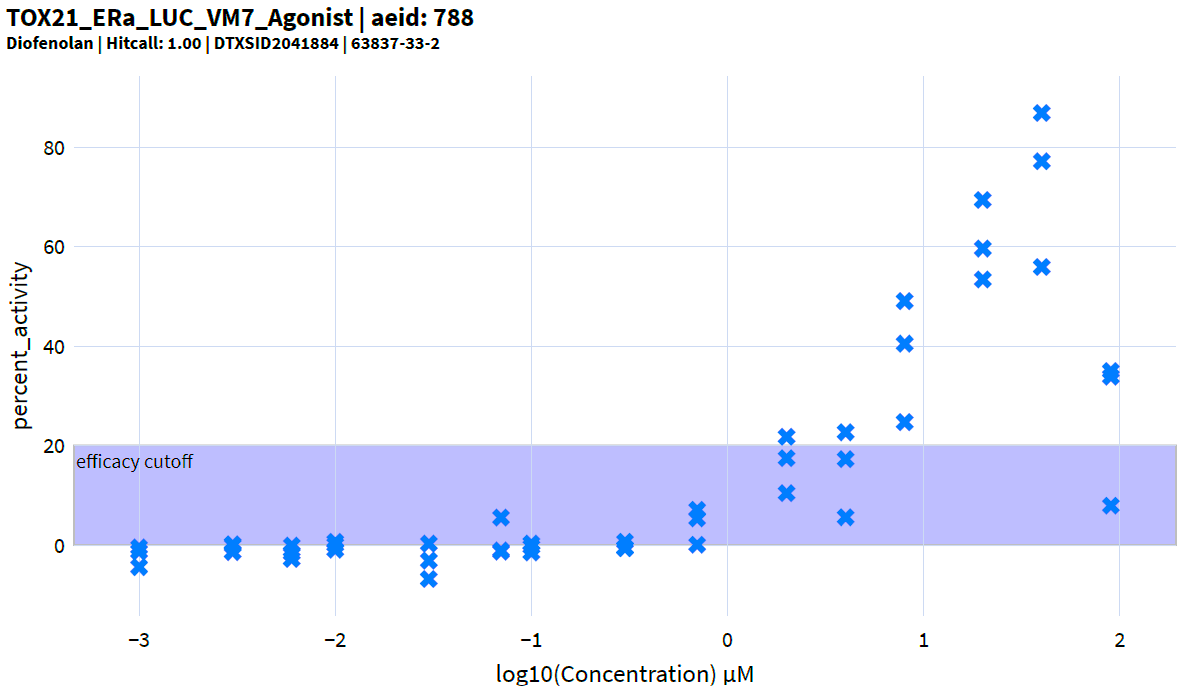
\includegraphics[width=1.0\textwidth]{figures/CRS.png}  
    \caption{The CRS belongs to \emph{Diofenolan} (DTXSID2041884), tested in the assay endpoint \emph{TOX21\_ERa\_LUC\_VM7\_Agonist} (aeid=788). The shaded region represents the estimated efficacy cutoff. This particular series comprises a total of $k = 45$ concentration-response pairs and is structured into $n_{conc} = 15$ distinct concentration groups, with each group consisting of $n_{rep} = 3$ replicates. }
~\label{fig:concentration_response_series} 
\end{figure}

In practice, concentrations are often subjected to multiple testing iterations, resulting in the distinct concentration groups with replicates. Table~\ref{tab:concentrations_quantities} presents the key quantities associated with an individual CRS when considering a specific assay endpoint $a_i$ and compound $c_j$. To visualize the variations in these quantities across the complete set of analyzed CRS in this work, please refer to Figure~\ref{fig:concentration_metric_distributions} in the Appendix. 

\begin{table}
    \centering
    \caption{Description of Parameters}
    \label{tab:concentrations_quantities}
    \begin{tabular}{ll}
        \toprule
        \textbf{Quantity} & \textbf{Description} \\
        \midrule
        $n_{\text{datapoints}_{i,j}}$ & Total number of concentration-response pairs ($|CRS|$) \\
        $n_{\text{groups}_{i,j}}$ & Number of distinct concentrations tested \\
        $n_{\text{replicates}_{i,j}}$ & Number of replicates for each concentration group \\
        $min_{\text{conc}_{i,j}}$ & Lowest concentration tested \\
        $max_{\text{conc}_{i,j}}$ & Highest concentration tested \\
        \bottomrule
    \end{tabular}
\end{table}

Concentration-response pairs, along with essential sample information such as well type and assay well-plate indices, can be retrieved by combining tables \emph{mc0}, \emph{mc1}, and \emph{mc3} from invitroDBv4.1, which represent the raw data. A special role is assigned to the control wells, which typically contain untreated samples or samples with a known, non-toxic response. They are used as a baseline to normalize the treated samples and account for any background noise in the assay~\cite{sheffield2021}. The concentrations are transformed to the logarithmic scale in micromolar, while the responses are control well-normalized to either fold-induction or percent-of-control activity:

\begin{enumerate}
    \item \textbf{Fold Induction}: is a measure used to quantify how much, for instance, gene expression has changed in response to a treatment compared to its baseline level from the control well set. E.g., if a gene is expressed five times higher in a treated sample compared to the control, the fold induction would be 5.
    \item \textbf{Percent of Control}: is another way to express the relative change in an activity due to a treatment compared to the control.
\end{enumerate}


\subsection{tcplFit2}\label{sec:tcplfit2}
\emph{tcplFit2}\footnote{\url{https://github.com/USEPA/CompTox-ToxCast-tcplFit2}} is an extension to tcpl, focused on curve-fitting and hit-calling. The package also offers a flexible and robust fitting procedure, allowing for the use of different optimization algorithms and the incorporation of user-defined constraints. This sets it apart from other open-source CRS modeling packages such as \emph{drc} and \emph{mixtox}, as it is explicitly designed for HTS concentration-response data.

\subsection{Curve Fitting}
Curve fitting involves the adjustment of mathematical models to best match observed data. Maximum Likelihood Estimation (MLE) is a statistical technique used to find parameter values that maximize the likelihood of observing the data within the model. The likelihood function represents the probability of observing the data given the model's parameters. The various curve fitting models investigated in tcplFit2 are summarized in Table~\ref{tab:tcplfit2_models} and visually presented in Figure~\ref{fig:tcplfit2_models}.

% \afterpage{
%     \clearpage % Insert a page break before the table and figure
\begin{table}
    \centering
    \begin{threeparttable}[b]
    \caption{tcplfit2 Model Details}
    % \renewcommand{\arraystretch}{0.1}
    \begin{tabular}{lll}
    \toprule
    \textbf{Model} & \textbf{Label} & \textbf{Equations\tnote{1}} \\
    \midrule
    Constant & constant & \(f(x) = 0\) \\ 
    Linear & poly1 & \(f(x) = ax\) \\ 
    Quadratic & poly2 & \(f(x) = a\left(\frac{x}{b} + {\left(\frac{x}{b}\right)}^{2}\right)\) \\ 
    Power & power & \(f(x) = ax^p\) \\ 
    Hill & hill & \(f(x) = \frac{tp}{1 + {\left(\frac{ga}{x}\right)}^{p}}\) \\ 
    Gain-Loss & gnls & \(f(x) = \frac{tp}{(1 + {\left(\frac{ga}{x}\right)}^{p})(1 + {\left(\frac{x}{la}\right)}^{q})}\) \\ 
    Exponential 2 & exp2 & \(f(x) = a\left(\exp\left(\frac{x}{b}\right) - 1\right)\) \\
    Exponential 3 & exp3 & \(f(x) = a\left(\exp\left({\left(\frac{x}{b}\right)}^{p}\right) - 1\right)\) \\
    Exponential 4 & exp4 & \(f(x) = tp\left(1 - 2^{-\frac{x}{ga}}\right)\) \\
    Exponential 5 & exp5 & \(f(x) = tp{\left(1 - 2^{-(\frac{x}{ga})^{p}}\right)}\) \\
    \bottomrule
    \end{tabular}
    \begin{tablenotes}
        \item [1] Constrained parameters: $a$: x-scale, $b$: y-scale $p$: gain power, $q$: loss power, $tp$: top, $ga$: gain (x), $la$: loss (x)
    \end{tablenotes}
~\label{tab:tcplfit2_models}
\end{threeparttable}
\end{table}

\begin{figure}
    \centering
    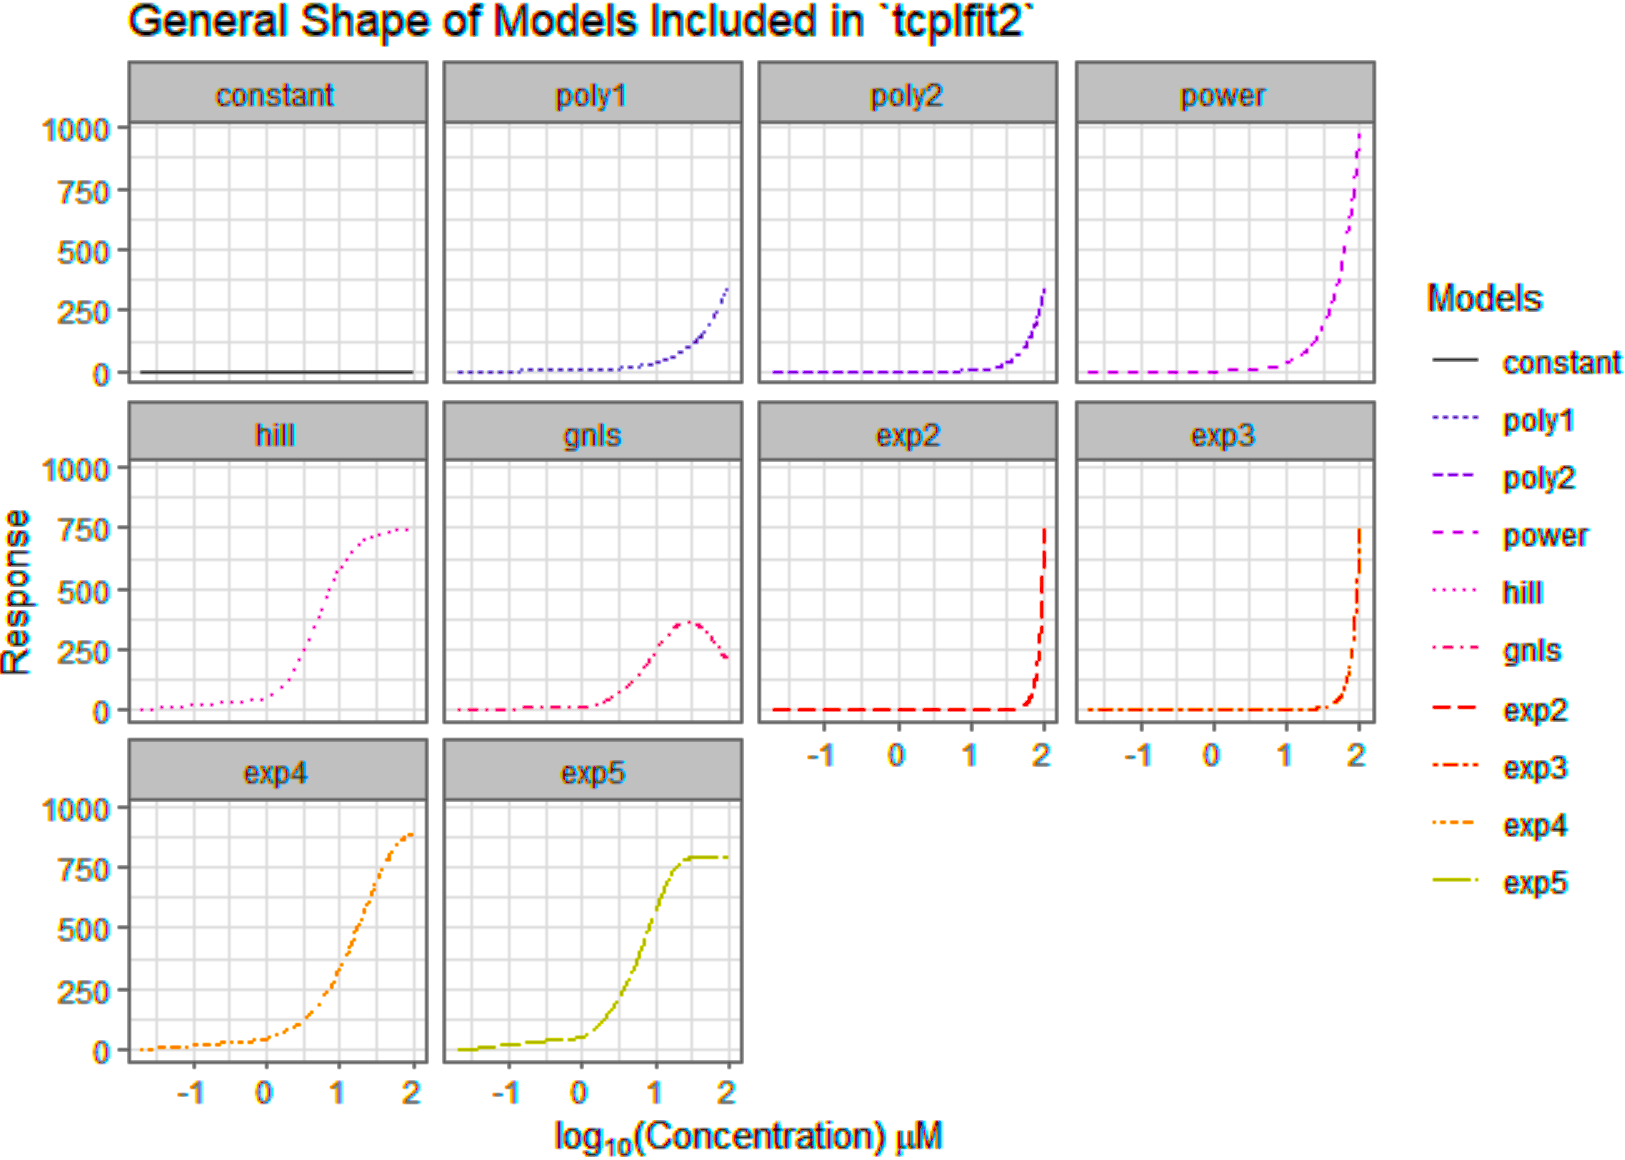
\includegraphics[width=1\textwidth]{figures/fit_models.png}
    \caption{Figure obtained from~\cite{tcplv3.0}.}
~\label{fig:tcplfit2_models}
\end{figure}

% \clearpage % Insert another page break after the table and figure
% }

In all models, it is presumed that the errors conform to a Student's t-distribution~\cite{tcplv3.0}. The presence of heavier tails in this t-distribution reduces the impact of outlier values, resulting in more resilient estimates compared to the frequently employed normal distribution. This robust model fitting approach eliminates the requirement for filtering out potential outliers before the fitting process. For a comprehensive explanation of the fitting procedure, please consult the official vignette\footnote{\url{https://cran.r-project.org/web/packages/tcpl/vignettes/Data_processing.html}}.

The \emph{Akaike Information Criterion (AIC)} serves as the metric for assessing the goodness of fit of models, defined by the formula: $AIC = -2\log(L(\hat{\theta}, y)) + 2K$, where $L(\hat{\theta}, y)$ is the likelihood of the model $\theta$ given the data and $K$ is the number of model parameters. The model with the lowest AIC value is chosen as the \emph{winning} model. The winning model is then used to estimate the efficacy and potency of the compound. The potency estimates, also called \emph{point-of-departure (POD)} estimates, are derived from the fitted curve, identifying certain \emph{activity concentrations (AC)} at which the curve first reaches certain response levels. Central POD estimates are depicted graphically in Figure~\ref{fig:active_and_pod}.

\begin{figure}
    \centering
    \begin{subfigure}[b]{0.48\textwidth}
        \centering
        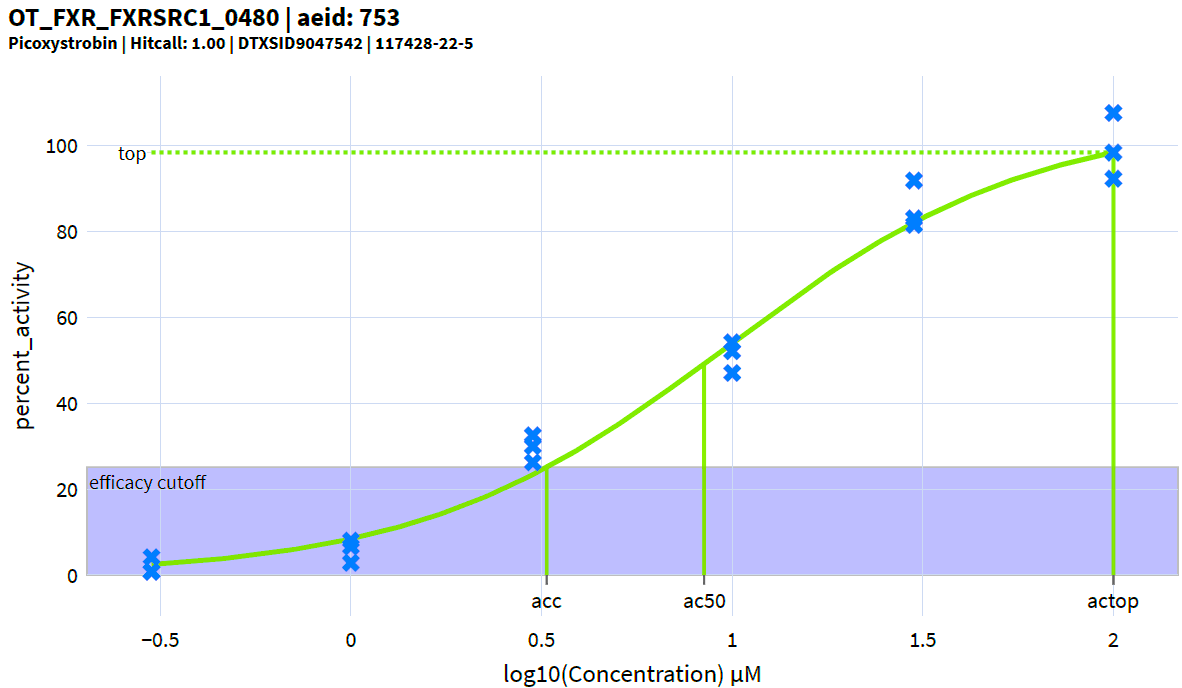
\includegraphics[width=\textwidth]{figures/POD.png}
        \caption{The Point of Departure (POD) (potency) estimates for the chemical \emph{Picoxystrobin} (DTXSID9047542) tested in the assay endpoint with $aeid=753$. The efficacy cutoff is defined at 25 percent-of-control activity. The winning fit model was the Hill function.~\emph{ACC}: The AC at the efficacy cutoff is $3.3 \mu M$.~\emph{AC50}: The AC at $50\%$ of the maximum response is $8.4 \mu M$.~\emph{ACtop}: The AC at the maximum response is $100 \mu M$.}
    ~\label{fig:active_and_pod}
    \end{subfigure}
    \hfill
    \begin{subfigure}[b]{0.48\textwidth}
        \centering
        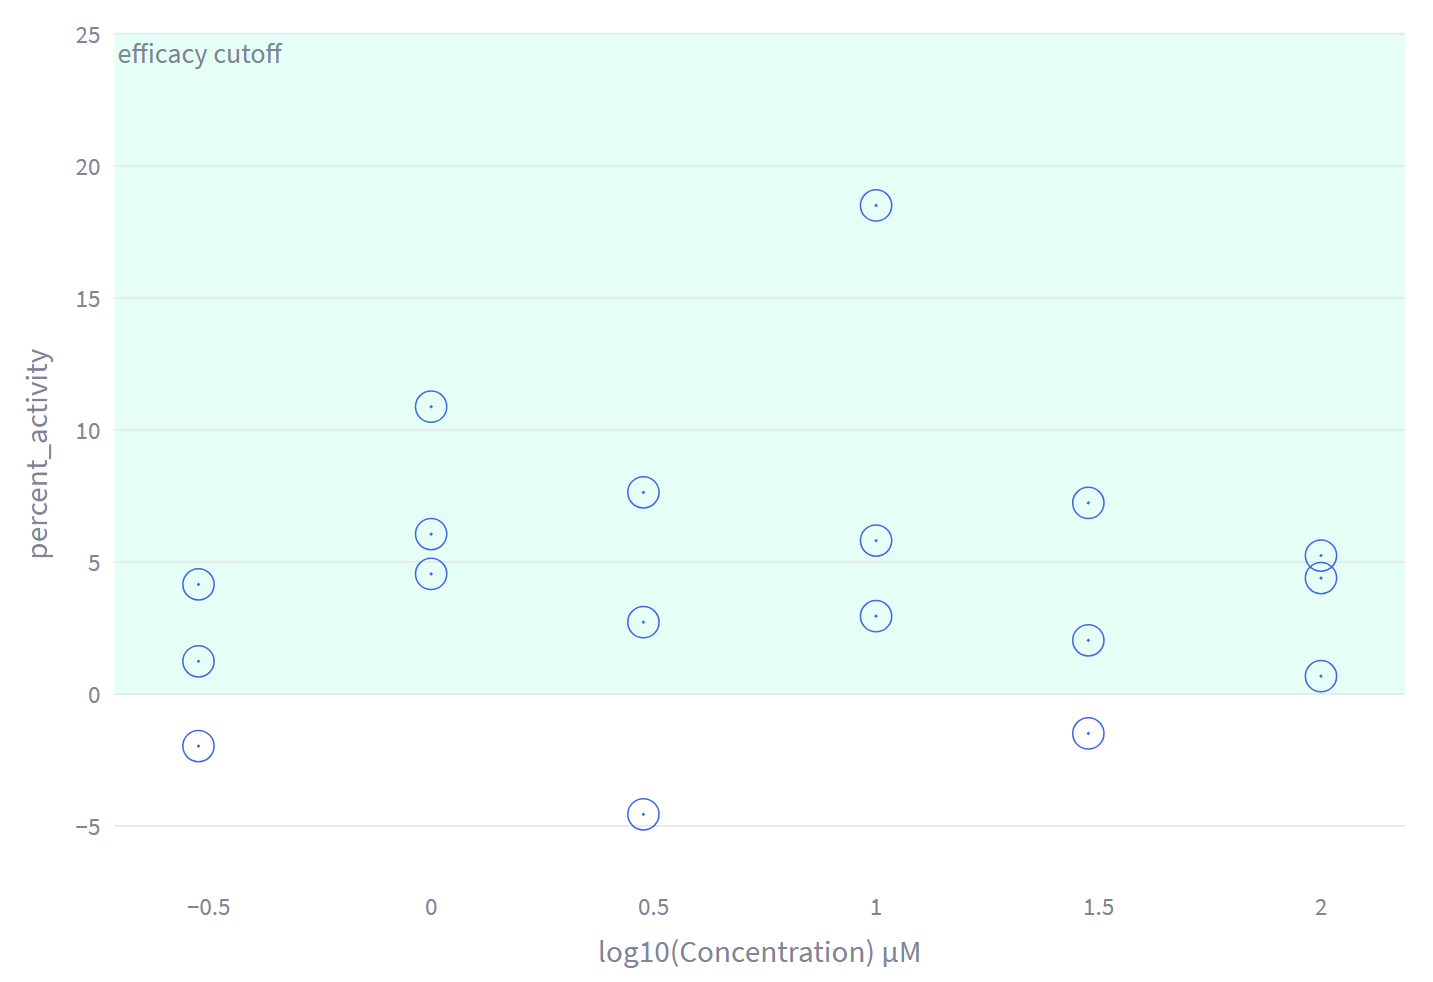
\includegraphics[width=\textwidth]{figures/inactive_and_no_pod.png}
        \caption{The Point of Departure (POD) (potency) estimates are not available for the chemical compound \emph{PharmaGSID\_48518} (DTXSID9048518), also tested in the assay endpoint with $aeid=753$. In this case, it was unnecessary as no response reached or exceeded $80\%$ of the efficacy cutoff, clearly indicating the inactivity of the compound. In such scenarios, a calculation of POD estimates is not applicable.}
        ~\label{fig:inactive_and_no_pod}
    \end{subfigure}
    \caption{Presence Matrix: assay endpoint-compound relationship.}
    ~\label{fig:pod}
\end{figure}


\subsection{Hit Calling}
A \emph{binary hitcall} hitcall simplifies the classification of the estimated activity for a specific compound tested in a particular assay endpoint and results in toxicity testing in a \emph{toxic} (hit) or \emph{non-toxic} (no hit) classification, often indicating whether the compound has reached a particular activity cutoff within a tested concentration range. It simplifies complex data into a straightforward result, making it easy to analyze and compare different compounds.

The \emph{continuous hitcall}, on the other hand, provides a more nuanced evaluation of the likelihood that a compound is active. The tcplFit2 package introduces a continuous hitcall, based on the product of the following three distinct probability values~\cite{sheffield2021}:

\begin{enumerate}[i.]
    \item that at least one median response is greater than the efficacy cutoff, computed by using the error parameter from the model fit and Student's $t$-distribution to calculate the odds of at least one response exceeding the efficacy cutoff;
    \item that the top of the winning fitted curve is above the cutoff which is the likelihood ratio of the one-sided probability of the efficacy cutoff being exceeded;
    \item that the winning AIC value is less than that of the constant model:
    \begin{equation}
    \frac{e^{-\frac{1}{2}AIC_{\text{winning}}}}{e^{-\frac{1}{2}AIC_{\text{winning}}} + e^{-\frac{1}{2}AIC_{\text{cnst}}} }
    \end{equation}
\end{enumerate}

In certain instances, compounds underwent multiple tests within a single assay endpoint, leading to their association with multiple CRS. In these exceptional cases, a hitcall is computed for each CRS, and then the highest hitcall value is recorded as the compound's ultimate hitcall.

\subsection{Flagging}
Finally, after processing, each CRS is assigned to an appropriate fit category based on the level of certainty in the estimated bioactivity. Additionally, cautionary flags are assigned to account for problematic data series or uncertainty related fits and hits.


\section{New Toxicity Pipeline Implementation: pytcpl}\label{sec:pytcpl}
\subsection{Introduction} 
This thesis introduces pytcpl\footnote{\url{https://github.com/rbBosshard/pytcpl}}, a streamlined \texttt{Python} repository inspired by the \texttt{R} packages tcpl and {tcplfit2}. This package was developed to accomodate customizable processing steps and facilitate interactive data visualization with an own \emph{Curve Surfer}\footnote{\url{https://pytcpl.streamlit.app/}}. The package optimizes data storage and generates compressed \texttt{Parquet} files of the relevant raw data and metadata from \emph{invitroDBv4.1}. Exclusively utilizing this repository eliminates the need for a complex and extensive database installation, rendering downstream analysis more accessible and efficient. It enables researchers who prefer \texttt{Python} to easily participate in data analysis and exploration, overcoming limitations associated with using \texttt{R} code.

The pytcpl pipeline adds an additional setup and post-processing step around the main pipeline:
\begin{itemize}
    \item \textbf{Setup}: This step involves user-specified subsetting of assay endpoints, tagging assays with external assay annotations, enabling workload balancing for distributed processing and generating \texttt{Parquet} files from all raw and metadata, optionally for database decoupled analysis.
    \item \textbf{Main} (similar to tcpl+tcplFit2): This step involves cutoff determination, curve fitting, hit calling and flagging.
    \item \textbf{Post-Processing}: This step has the goal of improving the overall quality of the data and involves post-processing curation, cytotoxicity interference reevaluation and the custom export of the final results.
\end{itemize}

\subsection{Setup step}\label{sec:subset_data}
\subsubsection{Subsetting Data}
For a better data comprehension, the presence matrix denoted as $P \in {\{0, 1\}}^{m \times n}$ is introduced. In this matrix, rows (indexed by $i$) represent assay endpoints $a_i$, and columns (indexed by $j$) indicate whether testing was performed (1) or not performed (0) for compound $c_j$ in those endpoints. Due to selective compound testing across different assay endpoints, the matrix $P$ is sparse. For a visual representation of the presence matrix $P$ covering all assay endpoints and compounds in \textit{invitroDBv4.1}, refer to Figure~\ref{fig:presence_matrix_all}.

\begin{figure}
    \centering
    \begin{subfigure}[b]{0.48\textwidth}
        \centering
        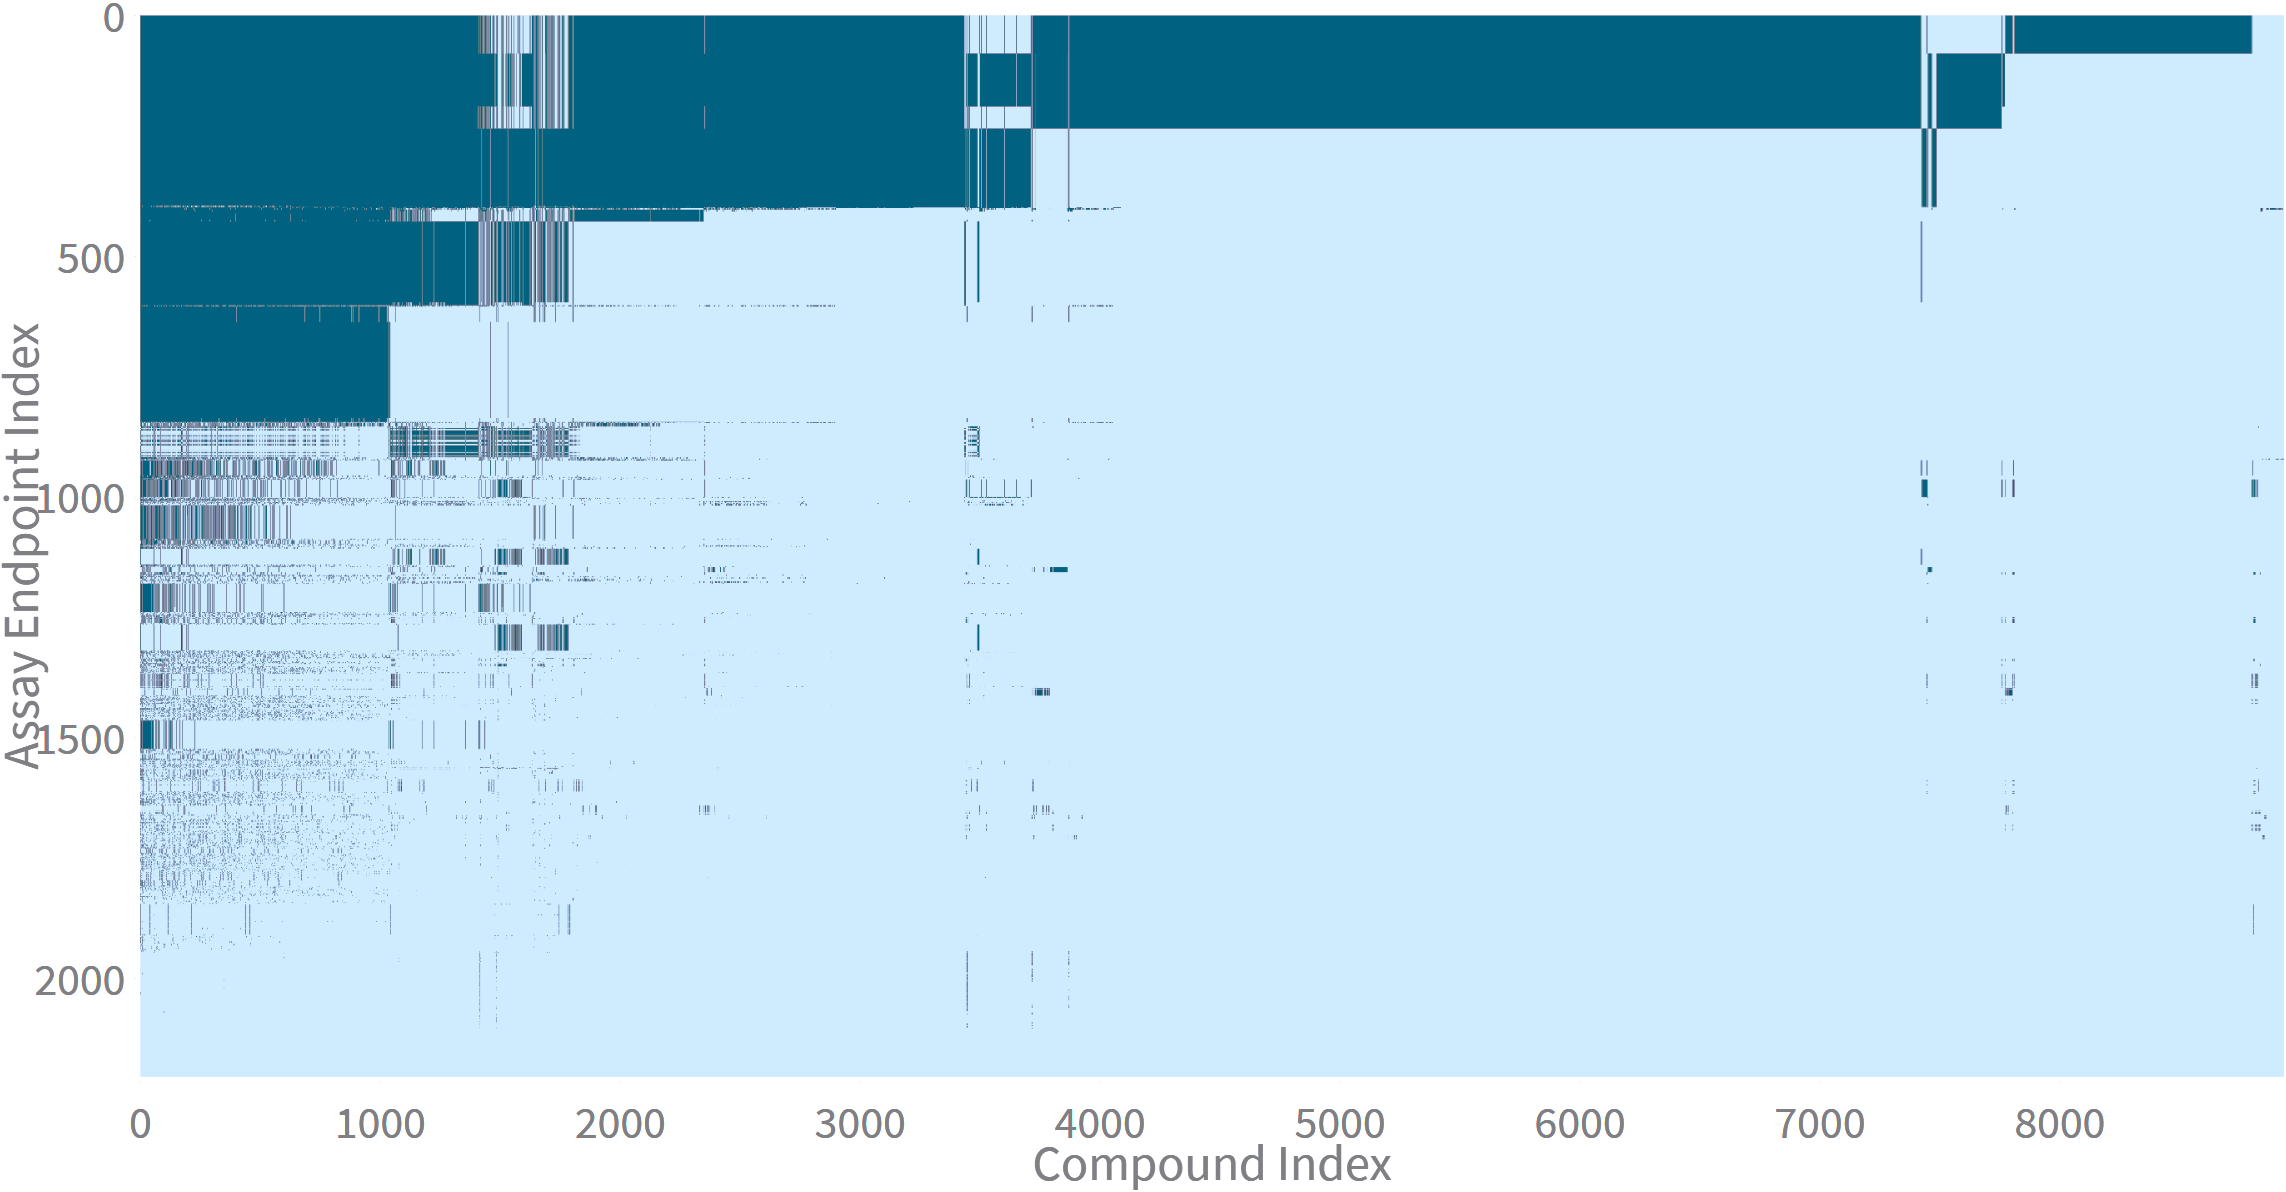
\includegraphics[width=\textwidth]{figures/presence_matrix_all.png}
        \caption{The presence matrix $P_{\text{all}}$, covers all assay endpoints and compounds from \emph{invitroDBv4.1}, totaling $m =$ 2'205 assay endpoints and $n =$ 8'935 compounds, excluding 606 compounds lacking molecular fingerprints. There are 3'196'178 concentration-response series available.}
    ~\label{fig:presence_matrix_all}
    \end{subfigure}
    \hfill
    \begin{subfigure}[b]{0.48\textwidth}
        \centering
        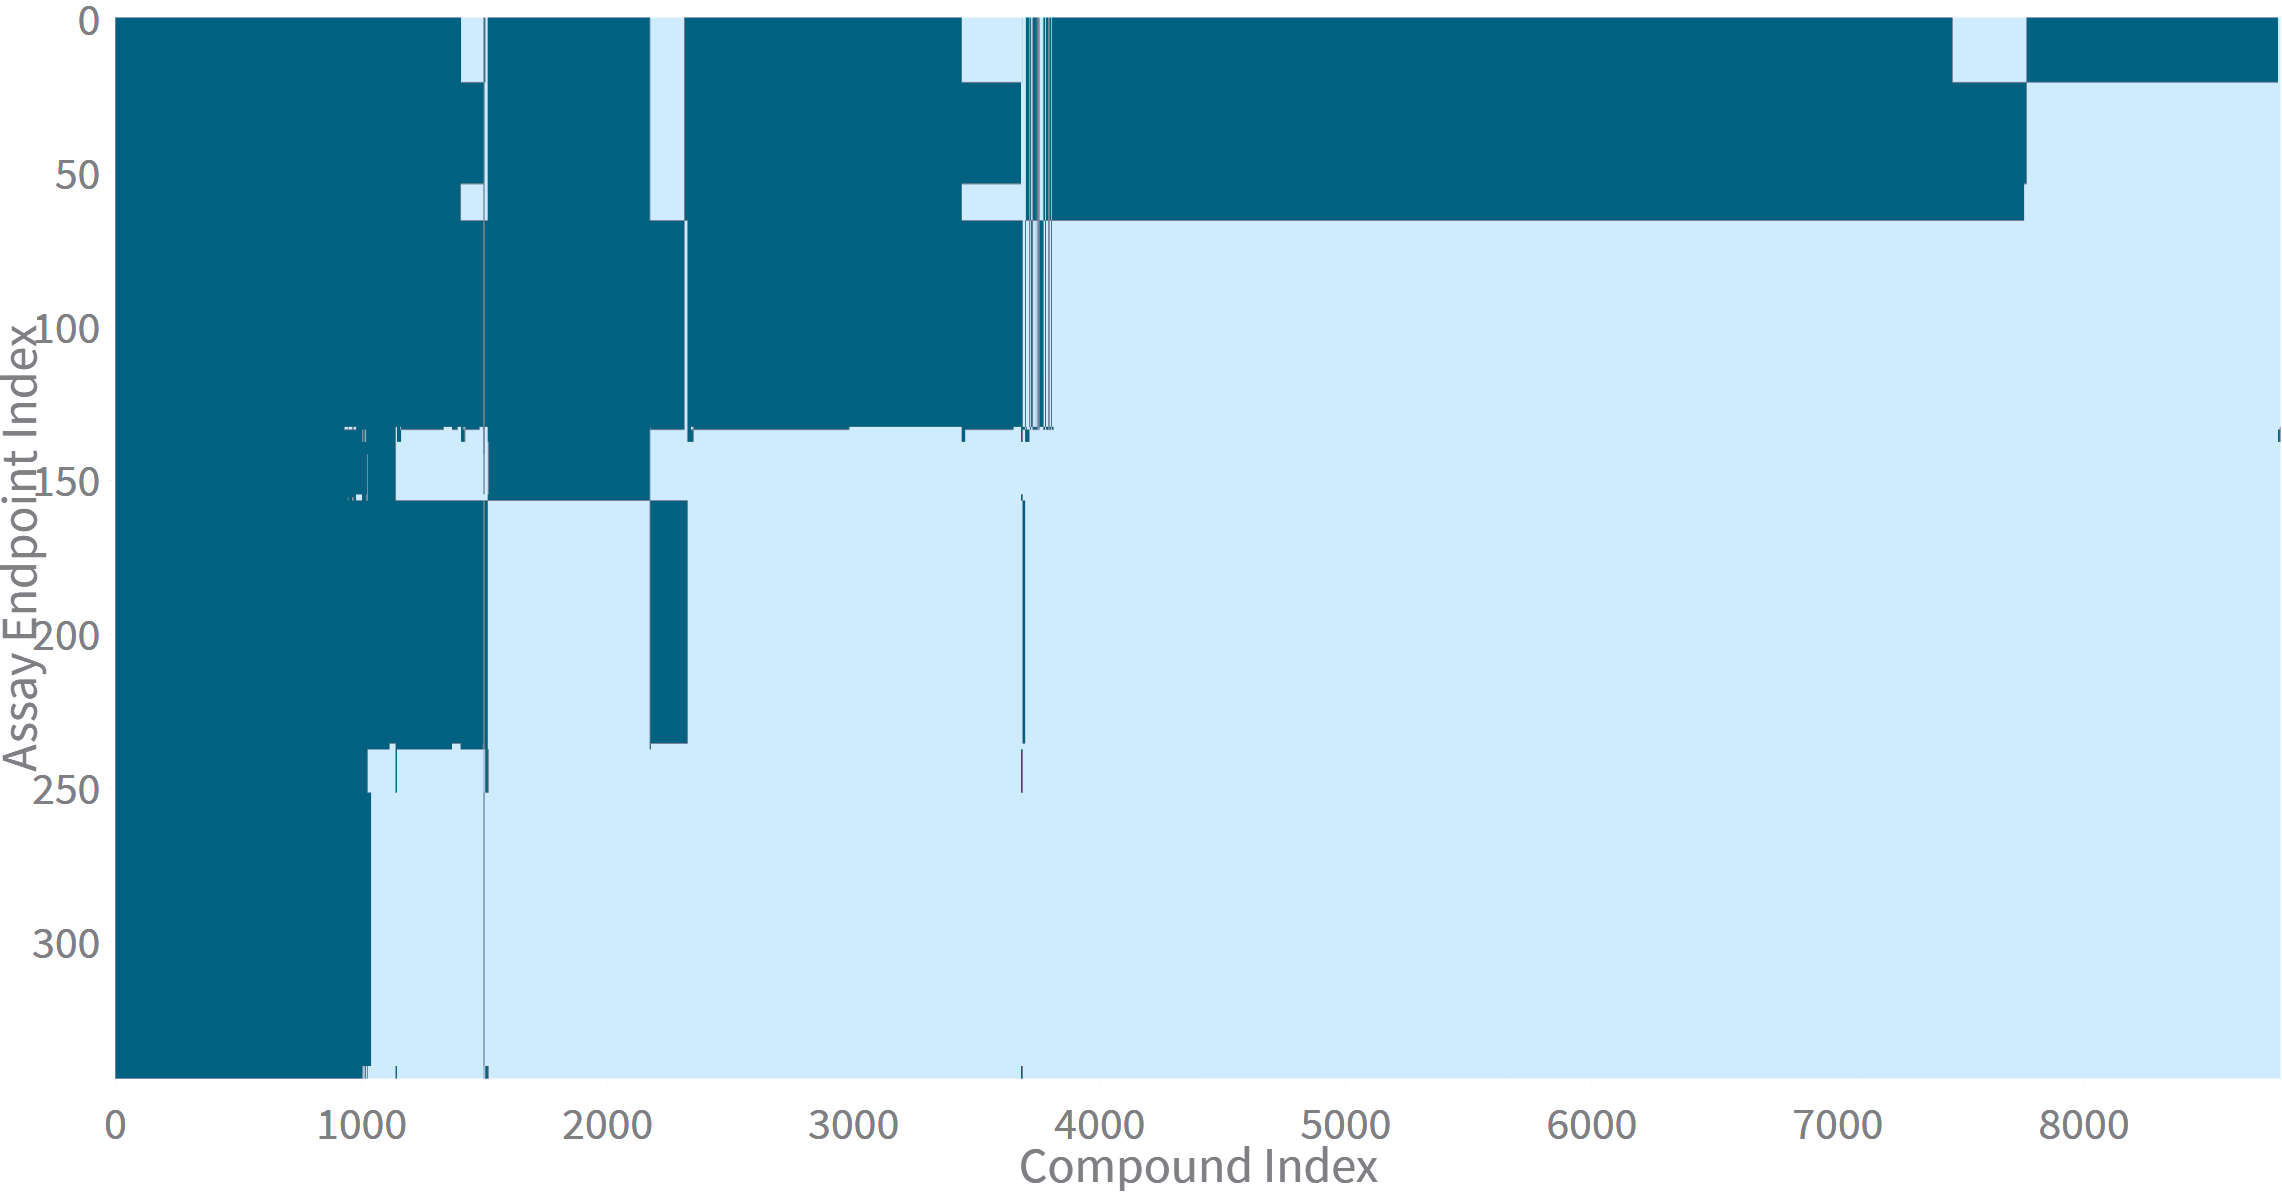
\includegraphics[width=\textwidth]{figures/presence_matrix_subset.png}
        \caption{$P_{subset}$ covers a specific subset of relevant assay endpoints and compounds considered for this thesis, totaling $m =$ 345 assay endpoints and $n =$ 8'804 compounds. Assay endpoints with less then 1'000 tested compounds were omitted. There are 1'043'222 concentration-response series available.}
        ~\label{fig:presence_matrix_subset}
    \end{subfigure}
    \caption{Presence Matrix: In both (a) and (b), structured by ranking according to the number of compounds associated with each assay endpoint, with compounds sorted in descending order
    of their occurrence frequency.}
    ~\label{fig:presence_matrix}
\end{figure}

In this thesis, we exclusively considered assay endpoints that have been tested with a minimum of $\num{1000}$ compounds. This selection criterion ensures the presence of adequate data for subsequent training of robust machine learning models. You can refer to Figure~\ref{fig:presence_matrix_subset} for a visual representation of the presence matrix $P$ which includes only this particular subset of assay endpoints. From this moment forward, we will refer to this specific subset as \emph{the} dataset, which will be the focus of this thesis. 

\subsubsection{Exernal Assay Annotation}
The assay endpoints were tagged with external annotations that involve the attributed toxcity endpoint, the type of mechanistic target and the mode of action.

The investigated assay endpoints are enriched with external annotations attributed by the Integrated Chemical Environment (ICE)~\cite{ice2022}, which provide valuable context and information about each endpoint. These annotations encompass the following aspects:

\begin{enumerate}
    \item \textbf{Toxicity Endpoint}: This annotation specifies the type of toxicity or adverse effect associated with each assay endpoint, helping to clarify the specific aspect of toxicity under investigation.
    
    \item \textbf{Mechanistic Target}: This annotation sheds light on the particular target mechanism or biological pathway being studied.
    
    \item \textbf{Mode of Action}: The annotations also describe how the tested compounds interact with the mechanistic targets and provides insights into the underlying biological processes or actions involved.
\end{enumerate}

\subsection{Main step}
The pytcpl main pipeline is similar to the \texttt{R}-based tcpl+tcplFit2 pipeline, with the exception of the curve fitting stage where the pytcpl pipeline made a notable modification by including a novel model the removal of the Exponential 3 model. The exclusion is a consequence of its infrequent selection as the winning model within the tcpl pipeline, indicating limited effectiveness in model fitting, as outlined in~\cite{feshuk2023}. Furthermore, an additional Gain-Loss 2 model was introduced during the curve-fitting stage. This model has one model parameter less than the Gain-Loss 1 model, which helps mitigate the risk of overfitting CRS data, making it less susceptible to outliers. Table~\ref{table:pytcpl_models} provides an overview of these changes within the pytcpl pipeline for reference.

\begin{table}
    \caption{pytcpl Model Updates}~\label{table:pytcpl_models}
    \centering
    \begin{threeparttable}[b]
    % \renewcommand{\arraystretch}{1.4}
    \begin{tabular}{llll}
    \toprule
    \textbf{Model} & \textbf{Label} & \textbf{Equations\tnote{1}} & \textbf{Role in pytcpl} \\
    \midrule
    Exponential 3 & exp3 & \(f(x) = a\left(\exp\left({\left(\frac{x}{b}\right)}^{p}\right) - 1\right)\) & Omitted \\
    Gain-Loss 2 & gnls2 & \(f(x) = \frac{tp}{1 + {\left(\frac{ga}{x}\right)}^{p}}\exp\left({-qx}\right)\) & New \\
    \bottomrule
    \end{tabular}
    \begin{tablenotes}
        \item [1] Parameters: $a$: x-scale, $b$: y-scale $p$: gain power, $q$: loss power, $tp$: top, $ga$: gain (x)
    \end{tablenotes}
\end{threeparttable}
\end{table}

\subsection{Post-Processing step}
\subsubsection{Post-Processing Curation}
Following the ICE guidelines\footnote{\url{https://ice.ntp.niehs.nih.gov/DATASETDESCRIPTION?section=cHTS}}, quality filters were implemented to enhance the processed concentration-response series. This step introduces OMIT/PASS curation warning flags, which could be applied either based on assay endpoints or compound quality control criteria.

\subsubsection{Cytotoxicity Interference Reevaluation}
As previously discussed in Chapter~\ref{chap:background}, the assessment of compound toxicity can be complicated by the presence of non-specific cytotoxic responses. In this section, we delve into the exploration of a method for reevaluating the reported hitcall status of active compounds, considering the estimated extent of cytotoxicity interference. The cytotoxicity of a compound in a target assay endpoint may be assessed by comparing the activity concentration at the efficacy cutoff, represented as $ACC_{\text{target}}$, with that of its corresponding viability assay endpoint counterpart (as exemplified in Table~\ref{fig:aeid_acid_aid}), referred to as $ACC_{\text{cyto}}$. 

\begin{table}
    \centering
    \caption{Each assay endpoint has an assay identifier (aid) used to match it with its viability counterpart that assesses cell loss. In this example, \emph{APR\_HepG2\_CellLoss\_24hr} (aeid=26) matches with aeid=38 and aeid=40. Similarly, \emph{APR\_HepG2\_CellLoss\_72hr} (aeid=46) matches with aeid=58 and aeid=60.}
    ~\label{fig:aeid_acid_aid}
    \begin{tabular}{|l|l|l|l|l|}
    \hline
    aeid & assay\_endpoint\_name & aid & assay\_name & assay\_function\_type \\
    \hline
    26 & APR\_HepG2\_CellLoss\_24hr & 3 & APR\_HepG2\_24hr & \textbf{viability} \\
    38 & APR\_HepG2\_P-H2AX\_24hr & 3 & APR\_HepG2\_24hr & signaling \\
    40 & APR\_HepG2\_p53Act\_24hr & 3 & APR\_HepG2\_24hr & signaling \\
    46 & APR\_HepG2\_CellLoss\_72hr & 4 & APR\_HepG2\_72hr & \textbf{viability} \\
    58 & APR\_HepG2\_P-H2AX\_72hr & 4 & APR\_HepG2\_72hr & signaling \\
    60 & APR\_HepG2\_p53Act\_72hr & 4 & APR\_HepG2\_72hr & signaling \\
    \hline
    \end{tabular}
\end{table}

If no counterpart is available in the database, we apply statistical approach to calculate a cytotoxicity estimate. It uses the median ACC for the compound of interest across a set of assay endpoints dedicated for capturing the cytotoxicity burst. 
The ACC is assumed to have a Gaussian error distribution. Cytotoxicity in terms of the respective potencies is assumed when: $ACC_{\text{cyto}} \leq ACC_{\text{target}}$. Thus, the probability of a compound being cytotoxic can be determined by

\[
P(\text{cytotoxic}) = P(ACC_{\text{cyto}} - ACC_{\text{target}} \leq 0) = \Phi\left(\frac{ACC_{\text{cyto}} - ACC_{\text{target}}}{\sqrt{\text{SD}_{ACC_{\text{cyto}}}^2 + \text{SD}_{ACC_{\text{target}}}^2 }}\right)
\]
    
where $\Phi$ is the Gaussian cumulative distribution function. The standard deviations $\text{SD}_{ACC_{\text{cyto}}}$ and $\text{SD}_{ACC_{\text{target}}}$ are unknown but are estimated as $0.3 \log_{10}$ ${\mu M}$ units~\cite{watt2018}. 

For the statistical approach with the cytotoxicity burst assays, $\text{SD}_{ACC_{\text{cyto}}}$ can be derived from the median absolute deviation (MAD) of the respective ACC values. Additionally, $P(\text{cytotoxic})$ is multiplied with the ratio of the number of cytotoxicity burst assay endpoints in which the compound exhibited activity ($n_{\text{hit}}$) to the total number of cytotoxicity burst assay endpoints in which the compound was tested ($n_{\text{tested}}$). 

Ultimately, $P(\text{cytotoxic})$ is then mulitplied with the original continuous hitcall of active compounds. The final cytotoxicity-corrected hitcall is then defined as follows: $\text{hitcall}_{\text{cyto-corrected}} = \text{hitcall}_{\text{original}} * (1 - P(\text{cytotoxic}))$.

\subsection{Curve Surfer}
Figure~\ref{fig:curve_surfer} presents the developed \emph{Curve Surfer}, a browser-based application that enables interactive data exploration and visualization of the processed data. The curve surfer tool is built using Streamlit, an open-source \texttt{Python} library that makes it easy to build custom web-apps for machine learning and data science. 

\begin{figure}  % Placement options: h (here), t (top), b (bottom), p (page)
    \centering
    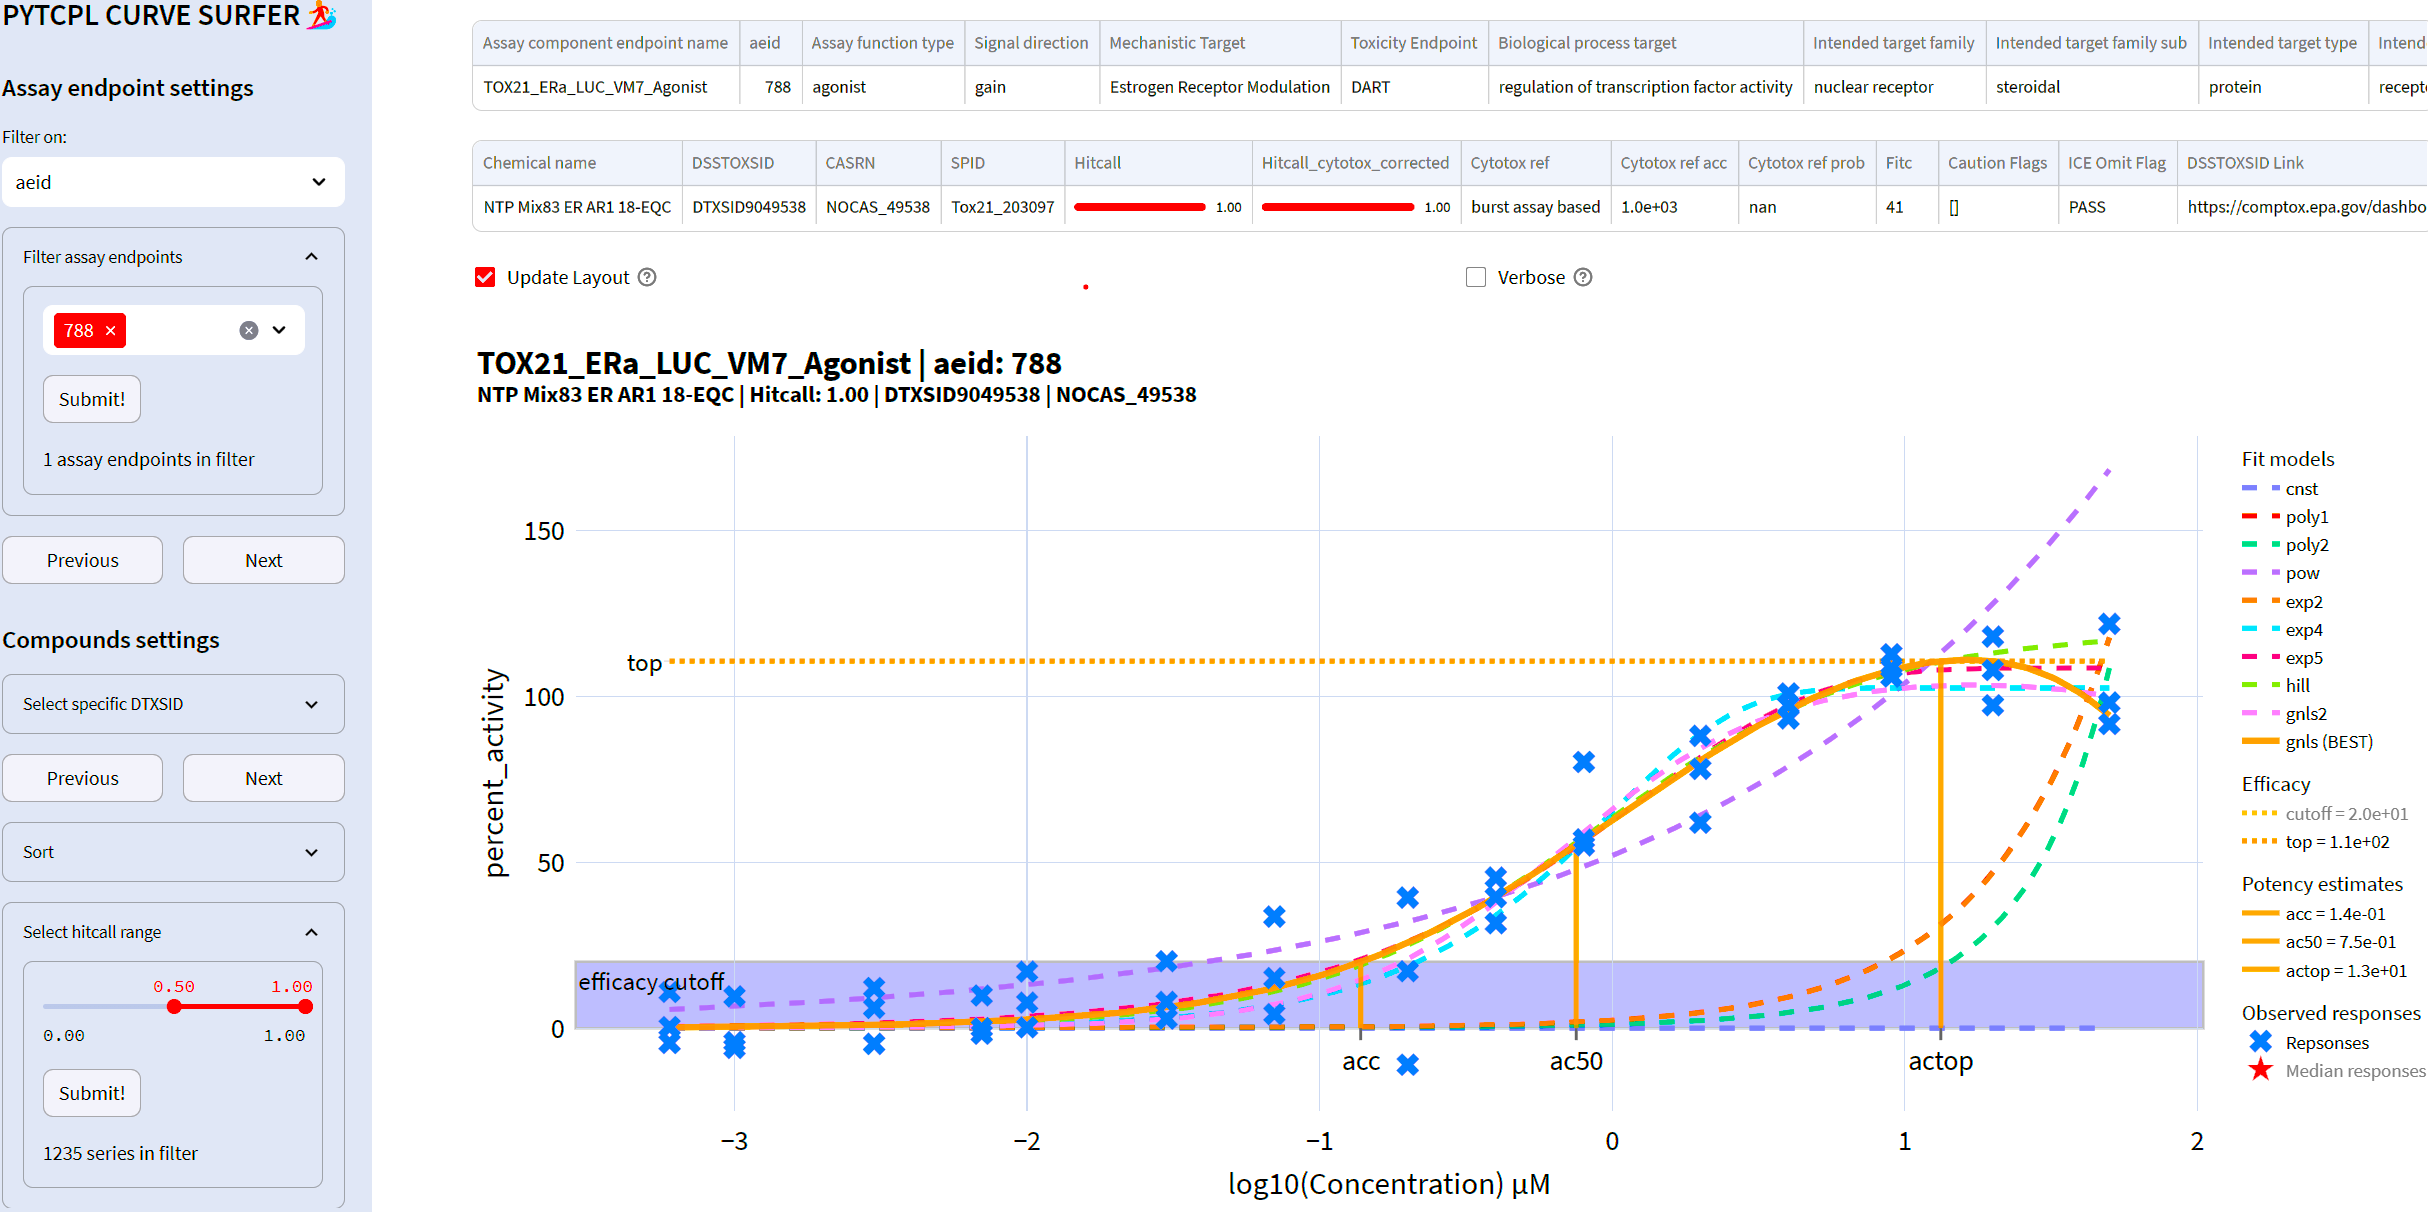
\includegraphics[width=1.0\textwidth]{figures/curve_surfer.png}
    \caption{The curve surfer provides the capability to narrow down assay endpoints based on critical annotations, and compounds can be selectively filtered using their DTXSID. Users can navigate through assay endpoints or the compounds within the current assay endpoint. Additionally, compounds can be filtered by their hitcall value or POD estimates using a range slider. Subsequently, the curve surfer displays comprehensive details for the chosen compound within the opted assay endpoint, showcasing CRS data along with curve fit models and metadata.}
~\label{fig:curve_surfer}
\end{figure}


\section{Toxicity Prediction from Molecular Fingerprints: Machine Learning Pipeline}
We employed distinct machine learning models for each assay endpoint, enabling the prediction of compound toxicity unique to each assay endpoint, coleveraging molecular structure inputs.
These models utilize molecular fingerprints to predict compound toxicity, as illustrated in Figure~\ref{fig:ml_dataset}. We applied both binary classification and regression models. In the case of binary classification, we use a threshold of $0.5$ to convert the continuous hitcall target values into binarized outcomes.

To create these individual datasets, we extract compounds that possess toxicity data for a given assay endpoint from the outputs generated by pytcpl. The associated hitcall values for these compounds are used as target variables within the machine learning model.

The binary input features for the model are molecular fingerprints with $2362$ bits derived from chemical structures. The structural data was obtained from the U.S. EPA's DSSTox database, accessed through the CompTox Chemicals Dashboard\footnote{\url{https://www.epa.gov/comptox-tools}}. The structural data mining and the necessary structure cleanup, as mentioned in Section~\ref{sec:toxicity_testing}, was conducted by Dr.\ Kasia Arturi\footnote{\url{https://gitlab.renkulab.io/expectmine/generating-fingerprints}}.

\begin{figure} 
    \centering
    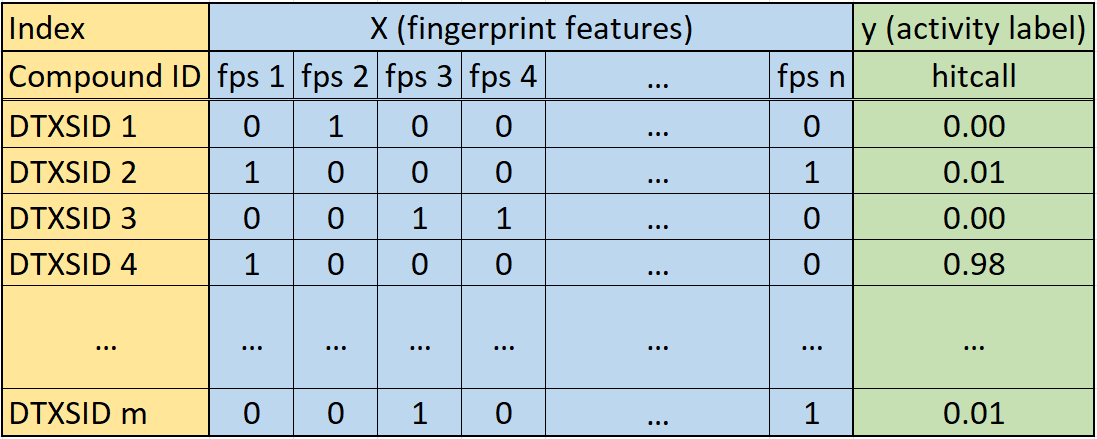
\includegraphics[width=0.8\textwidth]{figures/ml_dataset.png}
    \caption{Schematic example of a machine learning dataset related to a single assay endpoint. The dataset is structured into a feature matrix with $n=2362$ and a target vector. The feature matrix consists of molecular fingerprints, and the target vector is the hitcall value. For binary classification, the hitcall value is binarized based on a specific activity threshold (=0.5)}
~\label{fig:ml_dataset}
\end{figure}


The machine learning pipeline is structured into three main stages: model training, model evaluation and model application. The following sections and the diagram illustrated in Figure~\ref{fig:Project_overview} provide a detailed description of each stage.

\begin{figure}
    \centering
    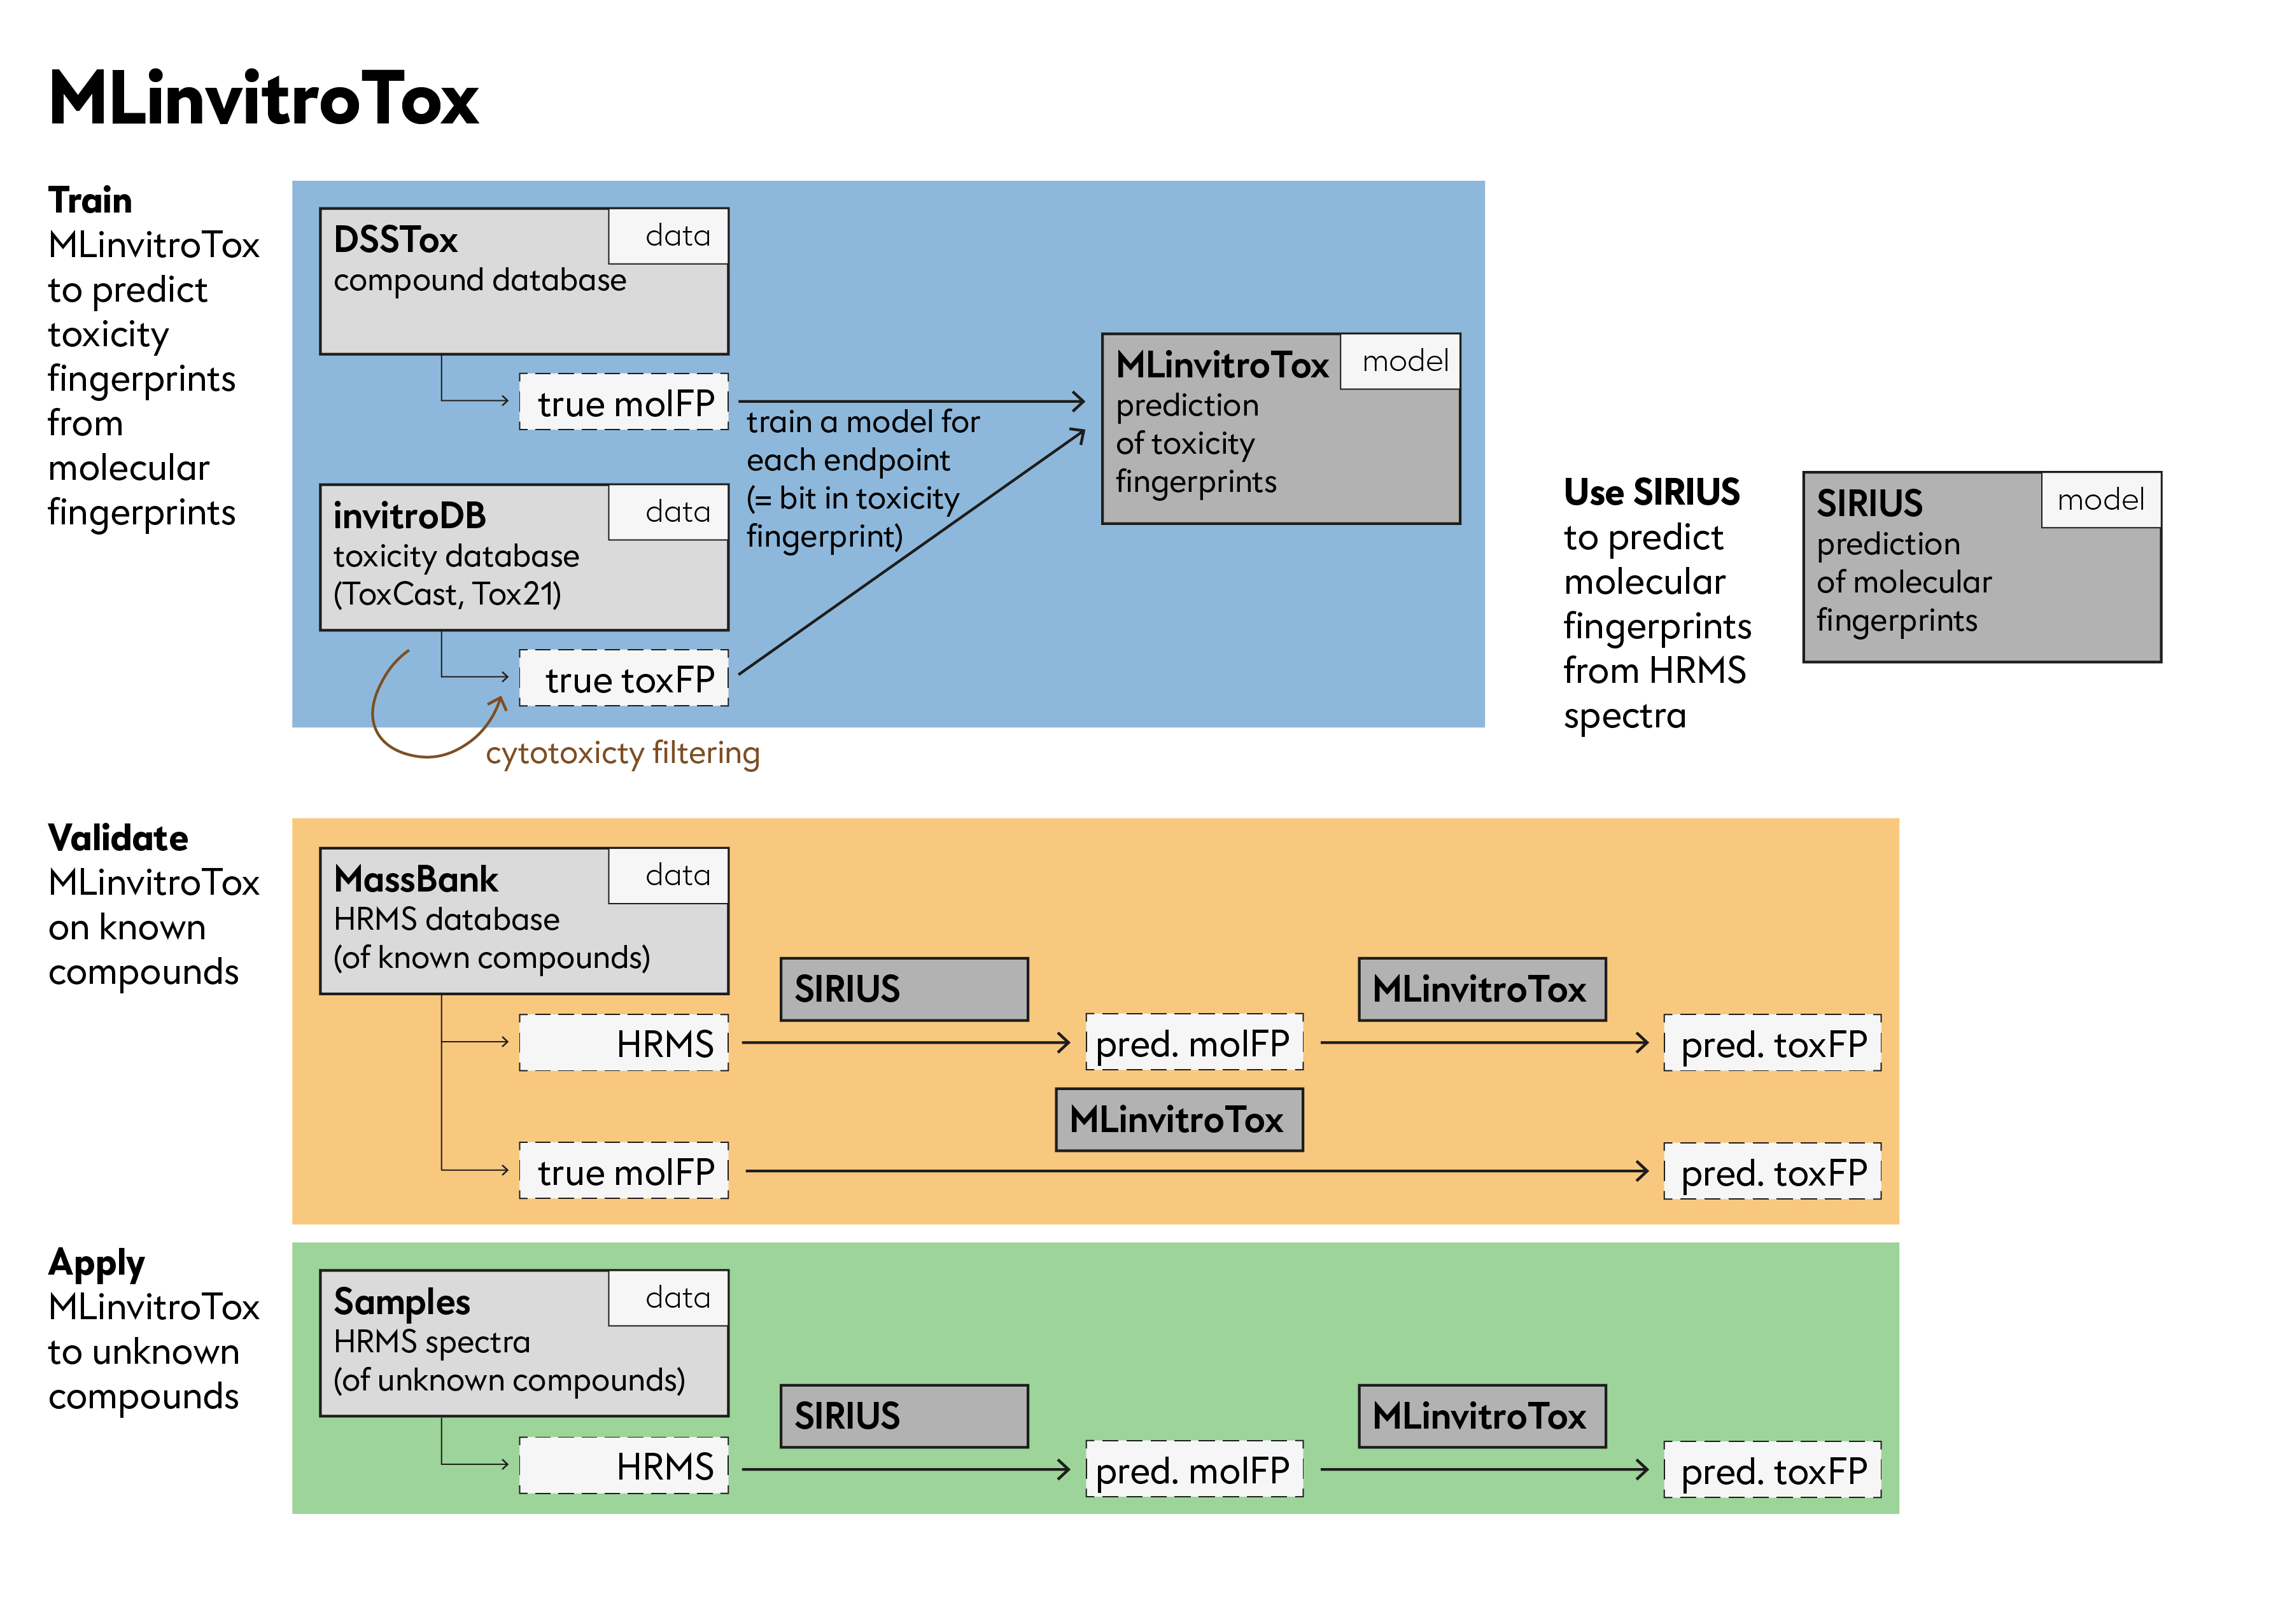
\includegraphics[width=1.0\textwidth]{figures/Project_overview.png}
    \caption{MLinvitroTox: Machine Learning Pipeline Steps. Figure created by Lili Gasser.}
~\label{fig:Project_overview}
\end{figure}

\subsection{Training}
The train stage is summarized in Figure~\ref{fig:Project_overview_train} and involves the generation of individual machine learning models for each assay endpoint. Each model is trained on a subset of the dataset with an 80/20 train-validation split. 

\begin{figure} 
    \centering
    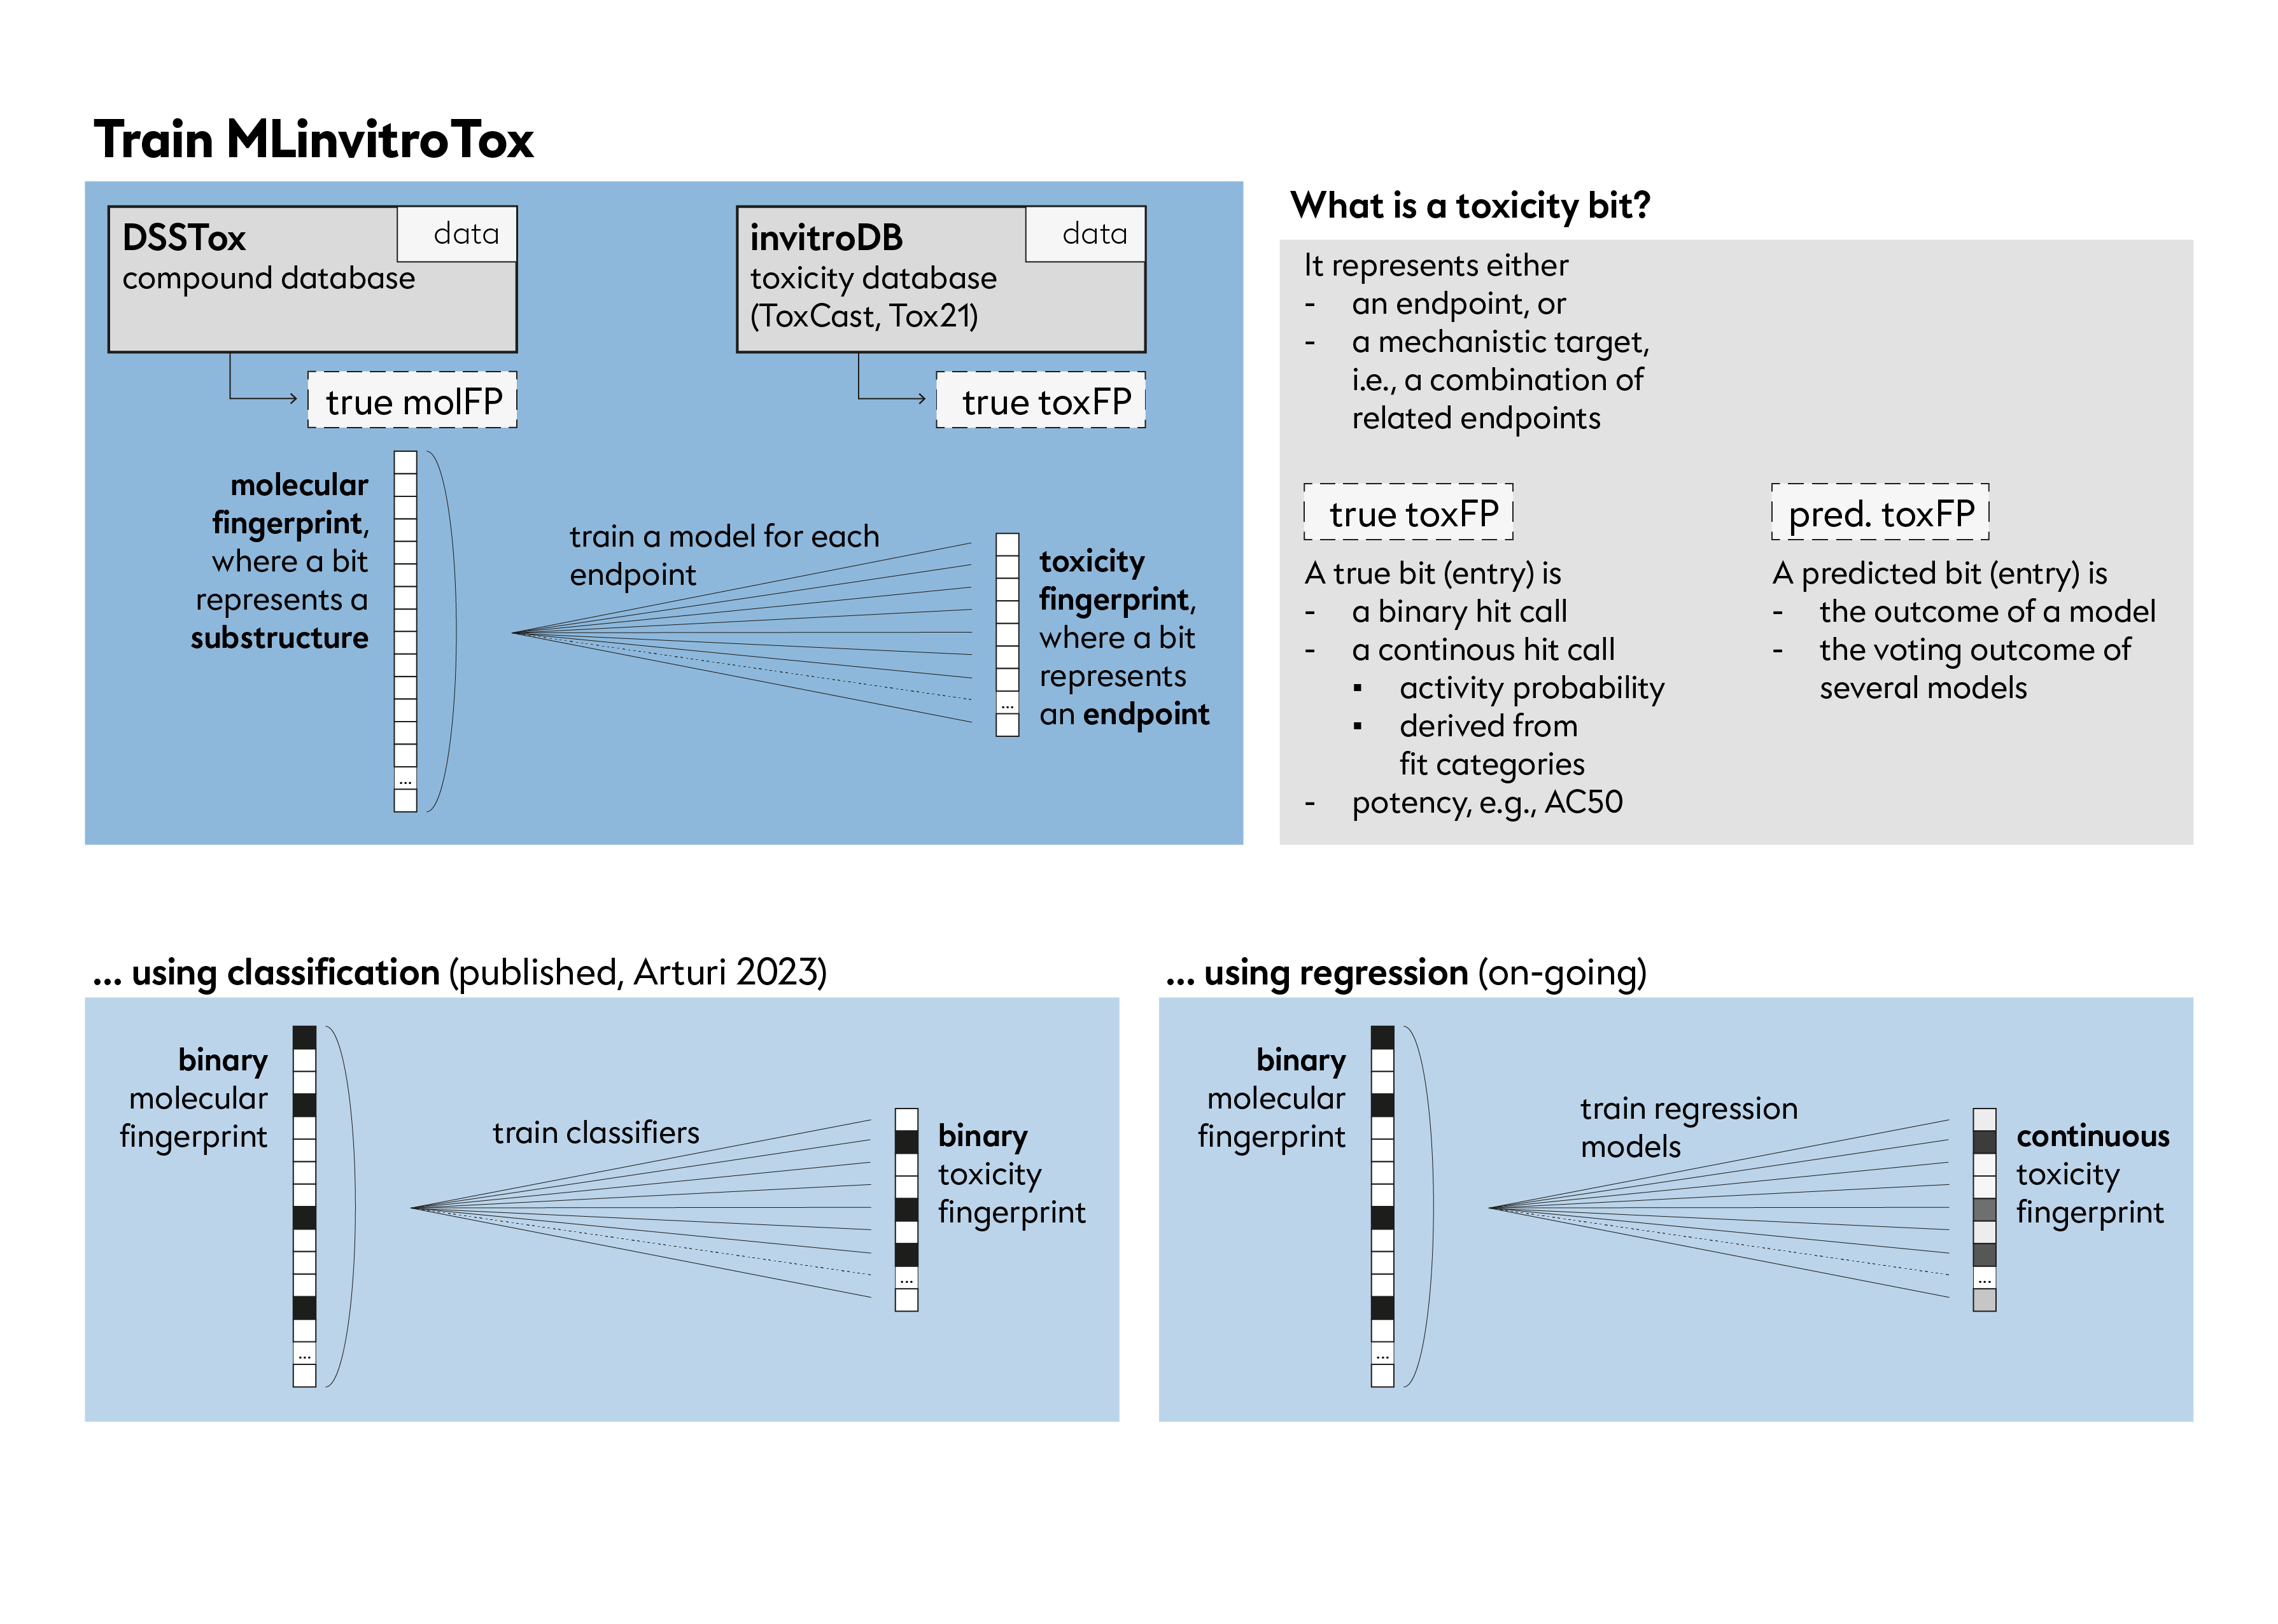
\includegraphics[width=1.0\textwidth]{figures/Project_overview_train.png}
    \caption{MLinvitroTox Train Step. Figure created by Lili Gasser.}
~\label{fig:Project_overview_train}
\end{figure}

\subsubsection{Feature Selection}
We applied feature selection\footnote{\texttt{sklearn.feature\_selection.SelectFromModel}} using either a xgboost or random forest model to narrow down the assay-endpoint relevant fingerprint features. The number of selected features is based on those features that exceed the mean feature importance threshold. All subsequent estimators are trained on these selected features.

\subsubsection{Model Selection}
The following supervised machine learning models from the \texttt{sklearn} library were considered: 
\begin{enumerate}
    \item \textbf{Logistic Regression} is a linear model that utilizes the logistic function to model binary dependent variables. It serves as a straightforward and interpretable model, often employed as a baseline for binary classification tasks.
    \item \textbf{Support Vector Machine} is a robust model with a lower susceptibility to overfitting and the ability to handle high-dimensional feature spaces.
    \item \textbf{Random Forest} is a bagging (bootstrap aggregating) ensemble learning technique that constructs a multitude of decision trees during training and combines their predictions, resulting in robust and accurate models with the advantage of reduced overfitting and the ability to handle high-dimensional data.
    \item \textbf{XGBoost} is a gradient boosting ensemble learning technique that combines multiple weak learner decision trees sequentially, with each new learner giving more weight to the examples that the previous learners struggled with. It provides typically high predictive accuracy and efficiency through techniques like gradient optimization and regularization.
    \item \textbf{Multi-Layer Perceptron} is a type of artificial neural network that consists of multiple layers of interconnected neurons and is used for various machine learning tasks, offering the advantage of modeling complex non-linear relationships in data.
\end{enumerate}

For every machine learning model, the selection process is based on a grid search over a set of hyperparameters, using 5-fold cross-validation. The hyperparameters, specified in a seperate config file, are optimized for binary classification based on the $\text{F}_{\beta}$ score, a generalization of the $\text{F}_{1}$. The $\text{F}_{1}$-score is the harmonic mean of the precision and recall and the more generic $\text{F}_{\beta}$ score applies additional weights, valuing one of precision or recall more than the other. We set $\beta=2$ to value recall higher than precision. 


\subsection{Evaluation}
To assess the performance of our trained models, we used two separate validation sets that were not part of the training data:

\begin{enumerate}
    \item The first straightforward validation set was used to evaluate how well the best estimator found by the grid search 5-fold cross-validation generalizes for unseen compounds. This set was randomly sampled from the tested compounds in the specific assay endpoints, ensuring that the number of active and inactive compounds was balanced.
    \item The MassBank validation set, as the second validation set, was used to evaluate the model's generalization capabilities, focusing on the domain gap between chemical structure space and fragmentation spectra. This validation set comprises compounds with both actual (from known structure) and SIRIUS-predicted fingerprints originating from MassBank spectra data. This dual fingerprint dataset enables the evaluation of the model's performance on both the actual and predicted fingerprints. In this context, the accuracy of SIRIUS framework's fingerprint predictions plays a critical role in assessing how well the model performs when applied to environmental samples. 

    It's important to highlight that compounds susceptible to data leakage, which were previously used in training the SIRIUS+CSI:FingerID prediction model (listed here\footnote{\url{https://bio.informatik.uni-jena.de/software/sirius/}}), have been excluded. If not excluded, the model's predictive capability for a compound's fingerprint would likely be very high because the model has already seen and learned from these data points during training. In the worst-case scenario, it could have essentially memorized the training data and the evaluation would become meaningless.

    After excluding these compounds, we are left with a potential upper limit of 429 compounds that can be safely used for MassBank validation. Nevertheless, the size of the MassBank validation set can differ among various assay endpoints due to variations in the overlap between the compounds tested in MassBank spectral data and those assessed in the assay endpoints, as depicted in Figure~\ref{fig:Massbank_validation}. Furthermore, Figure~\ref{fig:activity_ratio_comparison} provides an illustration of the distribution of hitcall representation in the validation set.
    
    
    \begin{figure}
        \centering
        \begin{subfigure}[b]{0.48\textwidth}
            \centering
            \includegraphics[width=\textwidth]{figures/Massbank_overlap.png}
            \caption{This figure illustrates across assay endpoints the count of compounds for which we possess both toxicity data and SIRIUS-predicted fingerprints from MassBank spectra. The range in the number of compounds in the MassBank validation set, which spans from 149 to 415, ist due to differences in the overlap with the compounds tested in the respective assay endpoints.}
        ~\label{fig:MassBank_overlap}
        \end{subfigure}
        \hfill
        \begin{subfigure}[b]{0.48\textwidth}
            \centering
            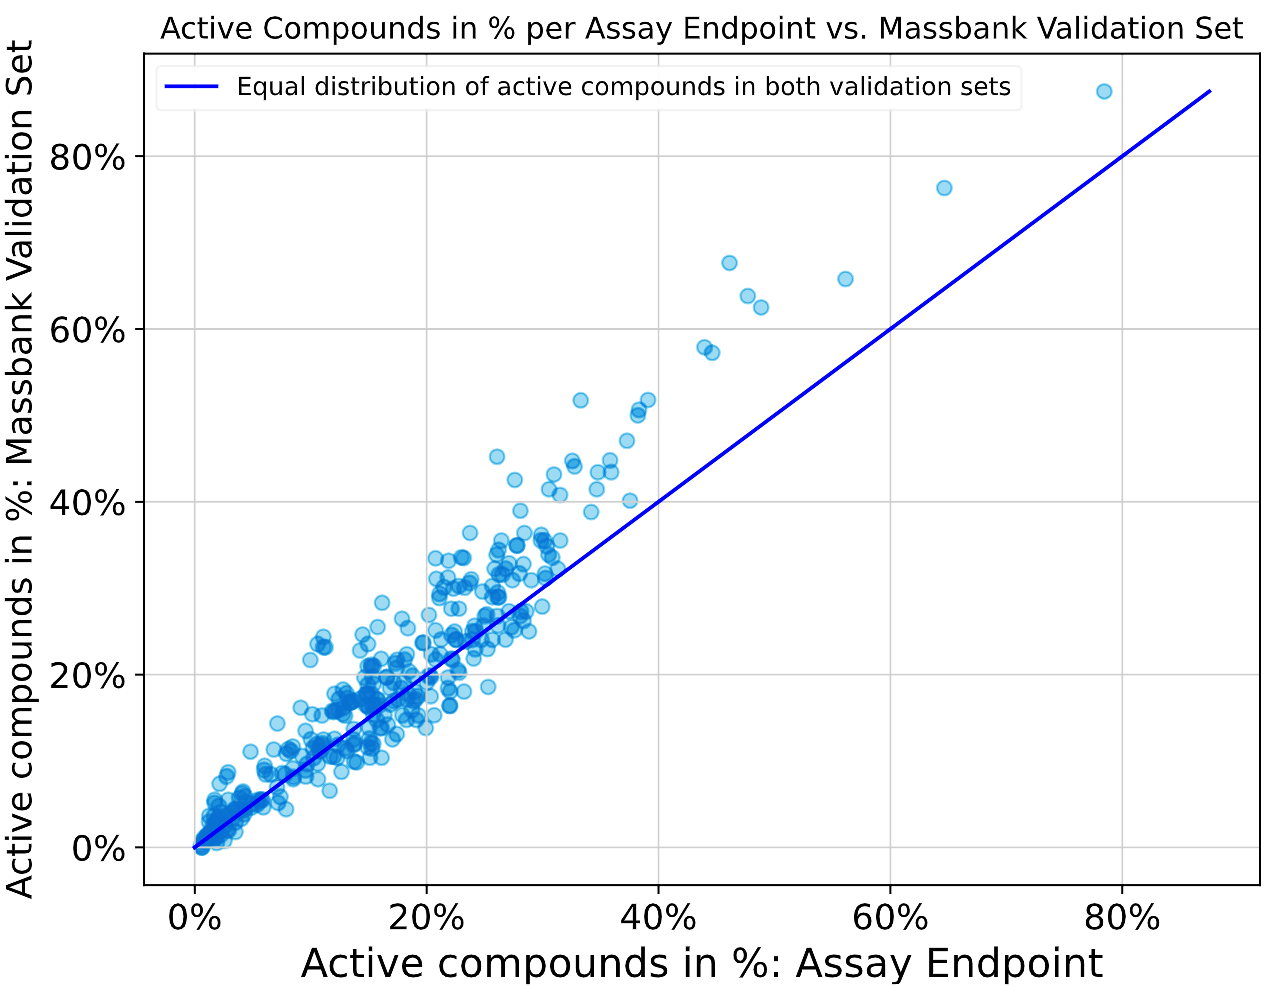
\includegraphics[width=\textwidth]{figures/activity_ratio_comparison.png}
            \caption{This figure plots the ratio of active (binarized) hitcall values for all compounds tested in the assay endpoint (x-axis) against the ratio of active (binarized) hitcall values for the compounds in the MassBank validation set (y-axis). The blue line represents the ideal case where the ratios are equal, and the validation set perfectly mirrors the entire dataset with respect to the target variable.}
            ~\label{fig:activity_ratio_comparison}
        \end{subfigure}
        \caption{MassBank validation set.}
        ~\label{fig:Massbank_validation}
    \end{figure}
\end{enumerate}


\subsection{Application}
The presence of distinct prediction models for each assay endpoint enables the grouping of these endpoints based on their annotations, such as the biological process or the mechanistic target annotation. This ultimately results in toxicity predictions averaged within these groups. These collective toxicity predictions are referred to as \emph{toxicity fingerprint} which serve the purpose of identifying the most toxic compounds for each specific assay endpoint.


